\documentclass[10pt]{article}
\usepackage{color}
\usepackage{palatino}
\usepackage{epsfig}
\usepackage[margin=1in,includefoot]{geometry}
%\usetikzlibrary{positioning}
%\usetikzlibrary{backgrounds}
\usepackage{paralist}
\usepackage{url}
\usepackage{alltt}
\usepackage{wrapfig}
%\usepackage{epsfig}
\usepackage{comment}
\usepackage{tabularx}
\usepackage{color}
\usepackage[font=small, labelfont={rm,bf}, margin=0.5cm]{caption}
\definecolor{williamspurple}{RGB}{89,23,128}
\definecolor{uclablue}{RGB}{50,132,191}

\topmargin=-0.5in
\oddsidemargin=0in
\evensidemargin=0in
\textwidth=6.5in
\textheight=9.0in

\pagestyle{empty}

\newcommand{\todo}[1]{\textcolor{red}{[#1]}}

\begin{document}
 \begin{Large}
\begin{center}
Coordination Plan
\end{center}
\end{Large}



We are aware that with 6 PIs and 2 Institutions, this NSF Large can degenerate into a set of 
separate projects thus losing the synergistic windfalls that come from truly working together as
a team. Our coordination plan rests on a foundation of existing collaboration between senior members,  technical leadership by the two young faculty in the two main technical thrusts and
congruent with their expertise and career trajectory, project leadership at the two
institutions by the two senior networking PIs, and at the most fundamental level by what we
call \emph{student bees}, students that are jointly advised by researchers at the two institutions who
can {\emph{cross-pollinate} the separate research projects.

\begin{enumerate}
\item \textbf{Foundation:} The two institutional leads, Govindan and Varghese, have worked
together since 2002 when they helped to advise Morley Mao (then at UCB, now at Michigan) on 
her thesis on route flapping (SIGCOMM 2002).  They worked together to supervise Harsha Govindan's thesis at UCSD on modeling routing table growth (SIGCOMM 2003).  Govindan and
Millstein have worked together since 2007 when network verification was not in vogue, combining 
Millstein's Programming Language expertise with Govindan's network experience through several
students including Ramakrishna Gummadi (now at Amazon), Nupur Kothari (now at Microsoft),
and Luis Pedrosa (now at EPFL).  The senior members at UCLA (Millstein-Tamir-Varghese) have been working together since 2016 when Varghese joined UCLA with regular weekly meetings for
the last year and co-advising of students Thomas Bui, Siva Kesava, and Allan Tang on network
verification.  

\begin{figure*}[htb]
\centering
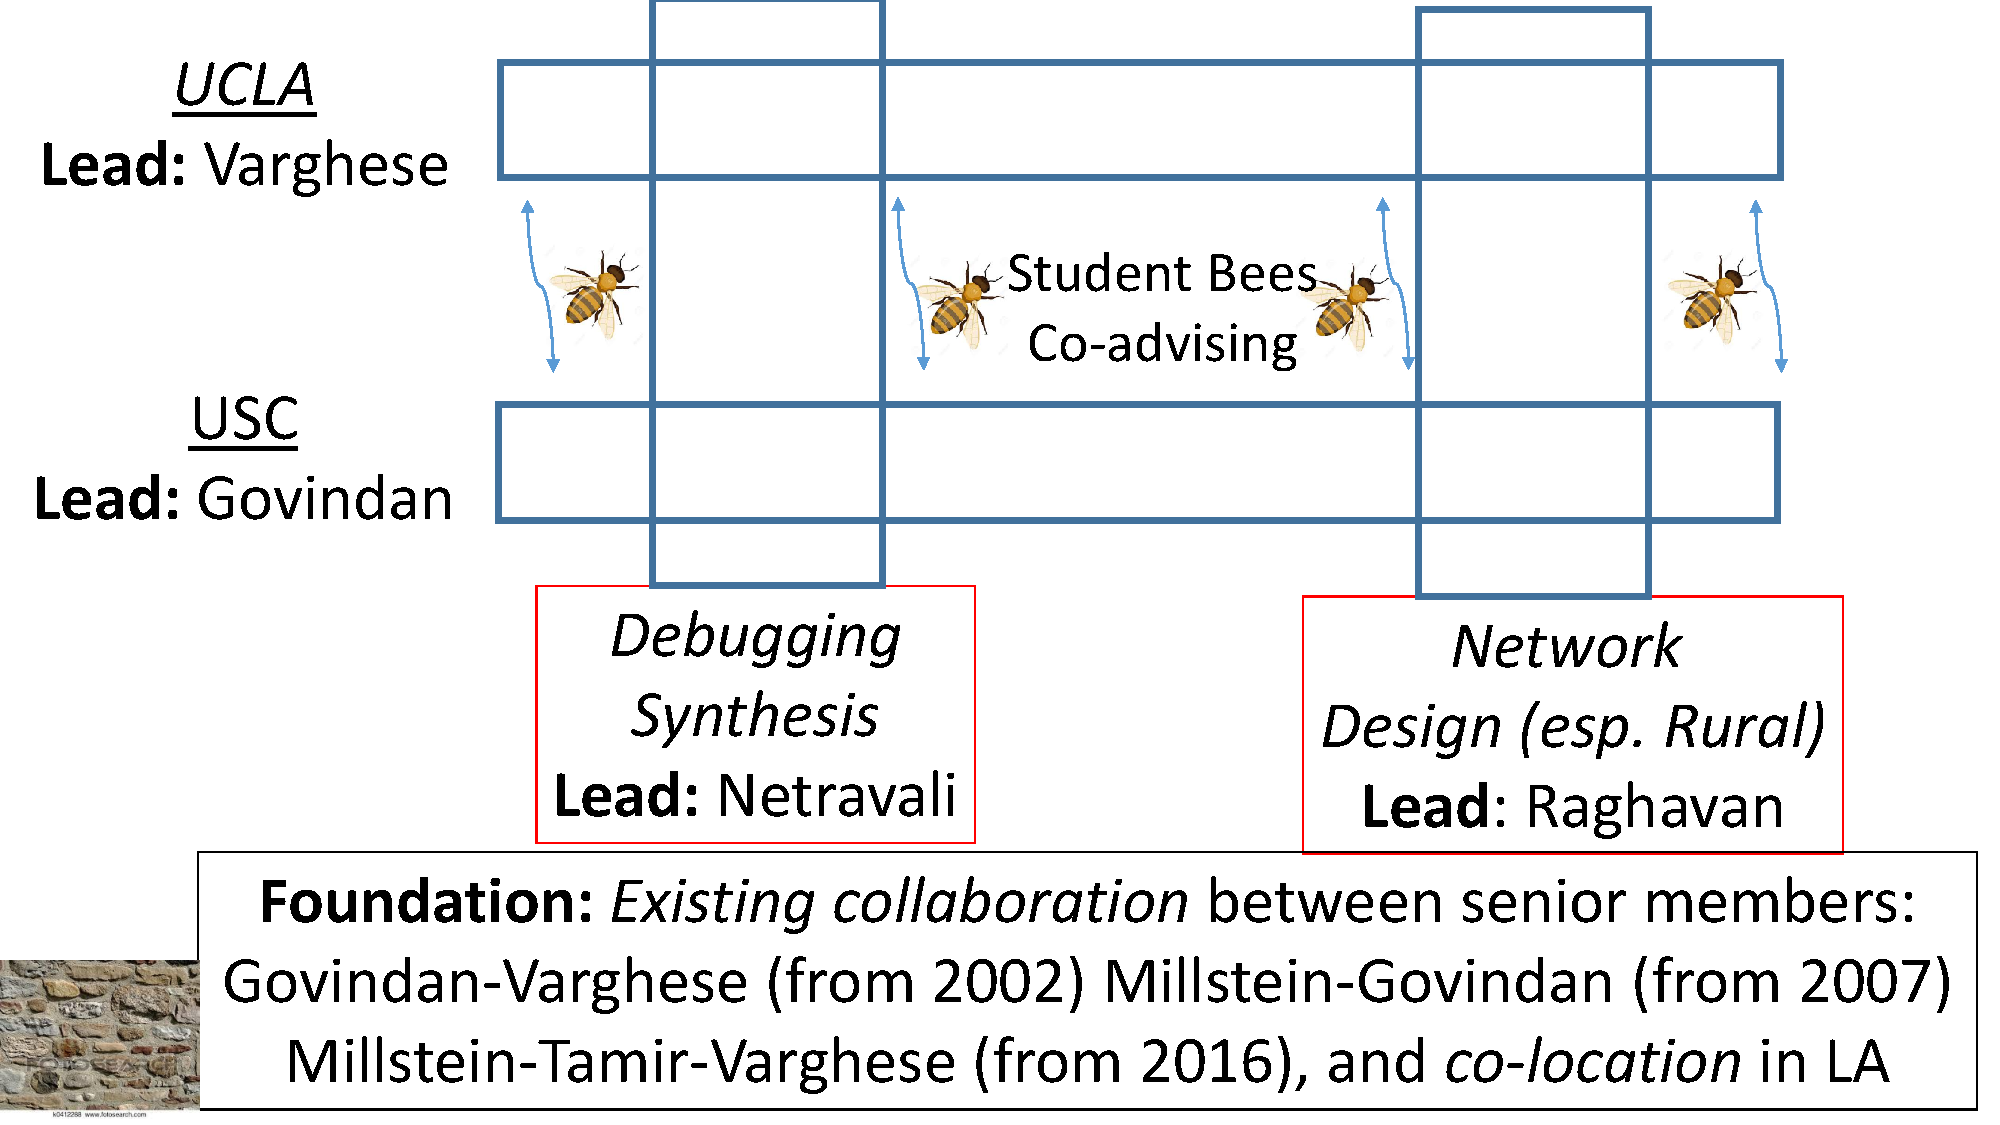
\includegraphics[width=0.7\textwidth]{coordinationplan.pdf}
\caption{Overview of our coordination plan to synergistically work across 6 PIs and 2 Institutions.}
\label{fig:overview}
\end{figure*}

\item \textbf{Technical Thrust Leaders:} Note that PI Netravali has just joined UCLA after his PhD at MIT with Hari Balakrishnan, and PI Raghavan has just joined USC after working for several
years with Shenker at ICSI in Berkeley. While each has a broad set of career directions, an important focus  focus for for Netravali is debugging and for Raghavan is rural networks. Netravali's PhD thesis was on web debugging and he has expertise in the complex systems interactions that
underly modern web systems, and his system Polaris for improving page load times has had
significant impact.  Raghavan has worked with Fred Kaufman the Technical lead
Motech and with David Hutchful the technical lead of Grameen for several years, and also
has contacts with Air Jaldi in India.  

Each is excited about leading and coordination their technical
thrusts across projects: Netravali will lead the project on mapping from operator concerns to
network DSL queries but he will participate the in the router primitive project with Tamir and
Varghese to  integrate from high level queries down  to router primitives.  He will also work
with Govindan and Varghese on automatically mining long term insights from operator logs which requires harnessing NLP as does the debugging thrust.

Raghavan will lead and coordinate the topology design (with Govindan and Varghese) and scripting (with Govindan, Millstein, and Varghese) starting with Motech and moving to Grameen.  Funds have been allocated for foreign travel to coordinate with Grameen and our collaborator Ashwin Gumaste in IIT Mumbai who will help us with a telesurgery application on his platform in IIT Mumbai.

\item \textbf{Institutional Leaders:} We will aim to start a Center for Network Design Automation
at UCLA and USC and ask for further input and support from Cisco, Google, Microsoft, and Huawei.
Varghese will coordinate the center at UCLA and Govindan at USC.  Between the two of them, they have over 40 years of experience and over 2 dozen successfully completed research grants, many
of which involved extensive (and often interdisciplinary) collaboration.  The institutional leaders
will meet with the technical leaders and the entire team of students and PIs once a month to ensure that the technical thrusts are being met and the overall project is coordinated.



\item \textbf{Co-advised Student Bees:} Ultimately, the life blood of the collaboration will the co-advised students based on our past experience of Mao, Narayan, Gummadi, Kothari, and Pedroso.  We will ensure that at least half our students are jointly advised by advisors from both USC and
UCLA.  The distance from UCLA to USC is only 14 miles; even with LA traffic this takes around 30 minutes for midday travel.  The past students of Govindan and Millstein (Gummadi, Kothari, Pedroso) spent significant time on both campuses, besides formal weekly project meetings.  
These students will be the bees that cross-pollinate the ideas in the projects.  For example, 
expertise in NLP, verification, rural networks is required across several projects, and the student
experts in each area can add great value to their colleagues in other projects.

\item \textbf{Project Leads:}  Each project within each thrust will have a project lead who is responsible for coordinating daily activities within each lead.  We will ensure that each PI will be the lead for at least one project.  For example, Millstein will lead the Network Verification
project, and Tamir will lead the Router Primitive project.

\item \textbf{Industry Feedback:} We will have an annual conference every two years (Year 1 at UCLA and Year 3 at USC) in the summer solicing industry feedback from a board comprised of Cisco, Google, Huawei, Microsoft, Motech and any other partners who join us later.  We will use the 
allocated workshop money for an outreach conference in network operations in Years 2 and 4 for underpresented and disadvantaged high school students (from East and South LA) at USC in
connection with the NAI-STEM program for first-generation college students at USC (of which Ragahav and Govindan are a part) and the BRAID initiative at UCLA (in which Millstein is an active paricipant).

\end{enumerate}



\end{document}
